\cotefile{147}
\scanpage{134}
\mspage{66}

termes, il faut introduire, \deleted{\unsure{des cas}}
pour un morphisme
\diagram{(218)\qquad
\begin{tikzcd}[ampersand replacement=\&]
\Delta_r \arrow[r,no head,"\alpha"] \& \Delta_{r'}
\end{tikzcd},}
un \uline{morphisme correspondant} de groupoïdes
\diagram{(219)\qquad
\fbox{\begin{tikzcd}[ampersand replacement=\&]
\widetilde{\Pi}_{\Delta_{r'}} \arrow[r,"\widetilde{\alpha}^{*}"]
\& \Pi_{\Delta_r}
\end{tikzcd}}}
qu'on appellera l'\uline{hom de générisation}
associé à $\alpha$.
\margin{\figure{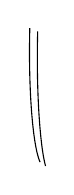
\begin{tikzpicture}
\draw (0,1.7) .. controls (-.02,.9) and (.04,.2) .. (.13,0);
\draw (.10,1.66) .. controls (.08,.9) and (.13,.2) .. (.20,-.05);
\end{tikzpicture}}}
Comme $\alpha$ se factorise
canoniquement en un hom surjectif
suivi d'un hom injectif de simplexes,
on est ramené à examiner séparément
les deux cas. Mais si $\alpha$ est surjectif
(``hom de dégénérescence''), \deleted{l'homomorphisme}
\inserted{on a $\alpha(0)=0$}
donc on est dans le cas déjà envisagé --
\deleted{\unsure{correspondant}}\inserted{d'ailleurs} dans ce cas
\diagram{\begin{tikzcd}[ampersand replacement=\&]
D^*_{\Delta_{r'}} \arrow[r] \& D^*_{\Delta_r}
\end{tikzcd}}
\unsure{se|a|à} décompose en des morphismes \unsure{:|;}
\diagram{(220)\qquad
\begin{tikzcd}[ampersand replacement=\&]
D^*_{d'_0,\unsure{\ldotp-\!-|-\!-},d'_{r'}}
\arrow[r] \&
D^*_{\unsure{d_0^{\deleted{\prime}}|d_0^*},-\!-,\unsure{d_r^{\deleted{\prime}}|d_r^*}}
\end{tikzcd},}
$(d_0,-\!-,d_r)$ est \unsure{déduite|déduit} de $(d'_0,-,d'_r)$
en \unsure{réécrivant} cette suite, en répétant certains
de ses éléments -- et \deleted{les} alors (220) est
un iso -- donc \uline{si $\alpha$ est un hom}
\margin{On voit que la considération des
$\widetilde{\Pi}_{d_0-d_r}$, $\Pi_{d_0,-d_r}$
pour $d_0,-\!-,d_r$ \unsure{non}
\unsure{\uline{strictement}|\uuline{strictement}}
décroiss. et celle de $\alpha^*$, pour $\alpha$
\unsure{non} \uline{stricts} croissants,
est de la poudre aux yeux, simplement !}
\margin{133}

